\section{Methoden} \label{sec:Methoden}
	
	\subsection{Aufbau}	
		
		\begin{figure}[ht]
			\centering
			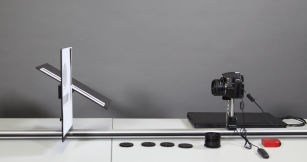
\includegraphics[width=0.8\textwidth]{bilder/aufbau.png}
			\caption{sample.\cite{WWU}} %TODO alex
			\label{fig:aufbau}	
		\end{figure}	
		Der Versuchsaufbau ist in Abb. \ref{fig:aufbau} dargestellt.
		Zu erkennen sind eine digitale Kamera und zwei Schirme, von denen einer verkippt liegt.
		Neben dem Objektiv auf der Kamera liegt ein weiteres mit einer Reihe an Blenden vor.
		
		Auf beiden Schirmen sind Testabbildungen aufgedruckt.
		Diese sind im Anhang in Abb. \ref{fig:testbild} dargestellt.
		
	\subsection{Kamera und Objektive}
	 
	 	Bei der Kamera, die verwendet werden soll, handelt es sich um eine Nikon D3200, auf der zunächst ein \SI{50}{\milli\meter} Nikkor Objektiv aufliegt.
		Das zweite Objektiv hingegen besteht lediglich aus einer Einzellinse mit einer Brennweite von \SI{60}{\milli\meter} auf welches verschiedene Blenden aufgeschraubt werden können.
		Diese besitzen einen Durchmesser von \SI{15}{\milli\meter}, \SI{7,5}{\milli\meter}-, \SI{3,75}{\milli\meter}.
		Zudem gibt es eine Lochblende, deren Blendendurchmesser bestimmt werden soll.
		
	\subsection{Grundlegende Theorie} \label{subsec:Theorie} %tempname
		
		Zuerst soll die Schärfentiefe $S$ an dem Nikkor Objektiv untersucht werden. 	
		Grundsätzlich kann nur die Fokusebene scharf auf die Bildebene abgebildet werden. 
		Punkte außerhalb dieser Ebene erscheinen als Zerstreuungskreise. 
		Solange diese klein genug sind, wird ein Objekt in dem Punkt noch als scharf wahrgenommen.
		In der Regel wird die Größe die dafür nicht überschritten werden darf als $Z = D_B/1500$ festgelegt.
		Dabei entspricht $D_B$ der Bilddiagonalen.
		
		Die kleinste Entfernung, ab der das Bild als scharf angesehen werden kann, heißt Nahpunkt. Entsprechend heißt die größte Entfernung, bis zu der das Bild als scharf angesehen werden kann, Fernpunkt. Die Schärfentiefe $S$ ist die Entfernung zwischen Nah- und Fernpunkt.
		
		Blenden vor oder hinter der Linse beeinflussen die Größe der Zerstreuungskreise. 
		Optische Auflösung wird durch die Eigenschaft eines Abbildungssystems, ein Objekt detailliert darzustellen, beschrieben. 
		Bei einer großen Blende (kleine Blendenzahl $k$) ergibt sich dadurch eine sehr kleine Schärfentiefe $S$, umgekehrt eine große für eine kleine Blende. 
		Die Auflösung verändert sich wie auch die Schärfentiefe $S$ durch den Durchmesser $D$ der Blende.
		
		Für jede gegebene Brennweite $f$ und Blendenzahl $k$ ergibt sich eine bestimmte Gegenstandsweite (bzw. Fokusentfernung), bei der sämtliche Gegenstände von dieser Weite bis ins Unendliche scharf abgebildet werden (d.h. der Fernpunkt liegt im Unendlichen). Diese Weite heißt hyperfokale Entfernung und spielt für die Berechnung der Schärfentiefe eine wichtige Rolle.
		Die hyperfokale Entfernung berechnet sich aus
		\begin{equation} \label{eq:hyperfokal}
			d_\text{h} = \frac{f^2}{k\cdot Z} + f = f \left( \frac{D}{Z}+1\right) .
		\end{equation}
		Der Nahpunkt errechnet sich für eine Gegenstandsweite $g$ durch
		\begin{equation} \label{eq:nah}
			d_\text{n} = \frac{g}{\frac{g-f}{d_h-f}+1}
		\end{equation} 
		und für den Fernpunkt:
		\begin{equation} \label{eq:fern}
			d_\text{f} = 
			\begin{cases}
				\frac{g}{\frac{f-g}{d_h-f}+1}, & \text{wenn } g < d_h \\
				\infty, & \text{wenn } g \geq d_h .
			\end{cases}
		\end{equation}
		
		Um die Schärfentiefe für das Nikkor Objektiv zu bestimmen, soll für acht verschiedene Blendenzahlen $k$ jeweils ein Foto von den Schirmen aufgenommen werden.
		Die Blendenzahl $k$ bestimmt sich durch das Verhältnis der Brennweite $f$ zu dem Blendendurchmesser $D$: 
		\begin{equation}
			k = \frac{f}{D}.
		\end{equation}
		Aus diesen Bildern soll die Bestimmung der Schärfentiefe subjektiv erfolgen.
		Dies wird erreicht, indem man die Zentimeterskala auf dem verkippten Schirm betrachtet und dem Foto entnimmt in welchem Bereich diese scharf zu erkennen ist.
		Hierfür soll der Satz des Pythagoras angewandt werden.
		Dabei gilt: $S^2 = d^2 - h^2$, wobei $S$ der Schärfentiefe, $h$ der Höhe des scharfen Bereichs auf dem Foto und $d$ der Bereich auf der Zenitmeterskala, der scharf wahrgenommen wird, entsprechen.
		Aus den Gleichungen \ref{eq:nah} und \ref{eq:fern} soll zudem die theoretische Schärfentiefe bestimmt werden und mit der subjektiven verglichen werden.
		
		Des weiteren sollen die Fotos mit dem Programm "ImageJ"\cite{ImageJ} und einem von der Universität bereitgestellten Plugin, welches MTF-Kurven anhand schräger Kanten berechnet, analysiert werden.
		Dabei steht MTF für "Modulübertragungsfunktion" und in Abhängigkeit der Raumfrequenz $\nu$ bestimmt sich eine MTF-kurve durch:
		\begin{align}
			\text{MTF}(\nu) = \frac{C(\nu)}{C(0)}, \quad C(\nu) = \frac{V_\text{max}-V_\text{min}}{V_\text{max}+V_\text{min}},
		\end{align}
		wobei $V_\text{max}$ gerade dem Grauwert einer großen weißen Fläche und $V_\text{max}$ dem Grauwert einer großen schwarzen Fläche entspricht.
		$C(\nu)$ gibt das Kontrastverhältnis an; Bei $\nu = 0$ ist dieses maximal.
		Als Qualitätsangabe eines Systems wird häufig der Wert angegeben, bei dem die MTF auf 50\% abgefallen ist.
		Dies soll für die acht verschiedenen Blendzahlen ermittelt und die erhaltenen Frequenzen gegen diese aufgetragen werden.
		Die Raumfrequenzen werden bei Digitalkameras in der Regel in lp/ph (Linienpaare pro Bildhöhe) angegeben, da so unterschiedliche Kamerasysteme und Objektive miteinander verglichen werden können, ohne auf die Vergrößerung zu achten.
		
		Eine direkte Bestimmung der MTF ist, unter Verwendung eines Testcharts mit Linienpaaren definierten Abstandes und definierter Breite, möglich.
		Mittels eines Profilplots senkrecht zu den Linienpaaren lässt sich der MTF-Wert für die räumliche Frequenz der aufgedruckten Linienpaare bestimmen.
		
		Für das zweite Objektiv, die Einzellinse, soll ebenfalls eine MTF pro Blende ausgewertet werden.
		Zudem soll auch eine alternative Methode zur Bestimmung der Auflösung betrachtet werden: Siemenssterne.
		Auf Abb. \ref{fig:testbild} sind zwei solcher Siemenssterne zu erkennen.
		Bei diesem speziellen Testmuster handelt es sich um einen Kreis mit abwechselnd weißen und schwarzen Sektoren.		
		In Richtung Mittelpunkt verringert sich der Abstand zwischen den Sektoren. 
		Die räumliche Frequenz der Linien nimmt also von außen nach innen zu. 
		Ab einem bestimmten Abstand kann der Stern nicht mehr aufgelöst werden und wird nur noch als graue Fläche wahrgenommen.
		Der Durchmesser $d_A$ dieser grauen Fläche ist ebenfalls ein Maß für das Auflösungsvermögen.
		Die Auflösung in Linienpaaren ergibt sich aus
		\begin{equation}
			l = \frac{\pi d_A}{n},
		\end{equation}
		wobei $n$ die Anzahl der Sektoren darstellt.
		Für diesen Versuch sind es 36.
		Zur Auswertung legt man zwei Linien durch den Mittelpunkt des Sterns und lässt sich die Grauwerte der Pixel unter den Linien ausgeben. 
		Eine Linie verläuft dabei durch zwei weiße Sektoren, die andere Linie durch zwei schwarze Sektoren.
		
		Die Ergebnisse beider Methoden sollen für das zweite Objektiv miteinander verglichen werden.
		
		Da das zweite Objektiv keine automatisch gewählte Belichtungszeit besitzt, soll zudem noch aufgetragen werden, wie sich die Belichtungszeit bei verschiedenen Blenden ändern muss, damit die Belichtung gleich bleibt.
		Für die Lochblende, bei der keine Größenangabe vorliegt, soll die Größe aus der Belichtungszeit bestimmt werden.
		
\section{Durchführung}
	
	Der Versuch wurde nach der Beschreibung in Abschnitt \ref{subsec:Theorie} durchgeführt.
	Dazu wurde die Kamera zunächst auf Werkeinstellungen zurückgesetzt. 
	Details wie die den Fotos zugehörigen Blendzahlen $k$ sind den Dateieigenschaften der einzelnen Bilder zu entnehmen.
	
	Während der Aufnahme einiger Fotos wurde auf dem Kameradisplay "Rauschreduzierung" angezeigt.
	% (Aufgrund des Umfangs dieses Berichtes wurden die aufgenommenen Fotos nicht angehängt)
	
	\subsection{Aufnahmen mit dem Nikkor Objektiv}
		
		Für die Blendzahlen $k=1,8$ und 2,8, 4, 5.6, 8, 11, 16, sowie 22 wurden je ein Foto von dem Testbild aufgenommen.
		Bei der Aufnahme dieser Fotos war die Kamera auf "Zeitautomatik" eingestellt, sodass die Belichtungszeit automatisch angepasst wurde.
		Damit beide Schirme auf den Fotos sichtbar wurden, wurde mit Hilfe der Liveview-funktion gearbeitet.
		Der Abstand der Kamera zu dem vertikalen Schirm betrug hierbei $g = \SI{102+-0,40}{\centi\meter}$.
		
	\subsection{Aufnahmen mit der Einzellinse}
	
		Hier wurden Fotos zunächst ohne Blende und dann für alle Blenden von beiden Schirmen aufgenommen und zusätzlich jeweils ein größeres Bild der Linienmuster aufgenommen.
		Durch Drehen des Objektivs, ließ sich der Fokus anpassen.
		Bei diesem Objektiv war keine Zeitautomatik möglich, weswegen die Belichtungszeit für die verschiedenen Blenden manuell eingestellt werden musste.
		Damit die Belichtung für alle Blenden gleich blieb, wurde die Belichtungszeit immer mit Hilfe von Histogrammen eingestellt.
		Diese Histogramme zeigten die Belichtung.
		Ihre Darstellung war eine der verschiedenen Kamerafunktionen.
		Neben der Belichtung der Kamera wurde für dieses Objektiv zusätzlich eine externe Lampe auf den Schirm gerichtet, damit dieser heller und somit die Kontraste besser zu erkennen waren. 
		Für diesen Versuchsteil war der Abstand zwischen den Schirmen und der Kamera $g = \SI{46,5+-0,40}{\centi\meter}$.
		
\section{Datenanalyse} \label{sec:Analyse}
	
	In diesem Abschnitt werden die Fotos ausgewertet.
	Die Betrachtung der Unsicherheiten erfolgt im Anhang.
	
	\subsection{Schärfentiefe bei dem Nikkor Objektiv}
		
		Zur Bestimmung der theoretischen Schärfentiefe $S$ musste zunächst die hyperfokale Entfernung bestimmt werden.
		Bis auf $Z$ bzw. die darin enthaltene Bilddiagonalengröße $D_B$ sind alle nötigen Variablen gegeben.
		Die Größe $D_B$ wurde mit Hilfe der Linien pro Millimeter auf den Testbildern den Fotos entnommen.
		Dazu wurde das Bildbearbeitungsprogramm "Gimp"\cite{Gimp} verwendet.
		Auf den Fotos entsprach \SI{1+-0,05}{\milli\meter} gerade $\frac 41/3 \approx 13,67$ Pixeln.
		Alle Fotos besaßen die gleichen Maße von 6016 x 4000 Pixeln.
		Daraus folgt eine Diagonale von $D_\text{B} = \SI{528,61+-26,43}{\milli\meter}$.
		Die Werte für die theoretische Schärfentiefe $S$ Ergibt sich durch
		\begin{equation}
			S = |d_\text{f}-d_\text{n}| = g\cdot (d_\text{h}-f) \cdot \left( \frac{1}{d_\text{h} - g} - \frac{1}{d_\text{h} + g -2f} \right),
		\end{equation}
		welche aus Einsetzen der Gleichungen \ref{eq:fern} und \ref{eq:nah} folgen.
		Diese sind in Tab. \ref{tab:Schärfentiefe_theo} aufgelistet.
		
		Die subjektiv empfundenen Schärfentiefen sind in Tab. \ref{tab:Schärfentiefe_subj} aufgefasst.
		Diese ergeben sich wie in Abschnitt \ref{subsec:Theorie} beschrieben aus $S_\text{sub}^2 = d^2 - h^2$.
		Dabei wurde $h$ aus der Pixelhöhe des scharfen Bereichs an der Zentimeterskala aus den Fotos entnommen und $d$ dem Abstand auf der Skala selber.
		Auch diese Größen sind in Tab. \ref{tab:Schärfentiefe_subj}.
		Da für die letzten beiden Blendzahlen $k$ die ganze Skala scharf zu erkennen war, wurde die subjektive Schärfentiefe $S_\text{sub}$ dort nur in einer Mindestgröße tabulliert.
			
		\begin{table}[ht]
			\centering
			\begin{tabular}{c|c|c|}
				$k$ & $d_\text{h}$ & $S$ \\
				\hline
				1,8 &  \SI{3.95+-0.20e+04}{\milli\meter} &  \SI{50.2+-2.5}{\milli\meter} \\
				2,8 &  \SI{2.54+-0.13e+04}{\milli\meter} &  \SI{78+-4}{\milli\meter} \\
				4 &  \SI{1.78+-0.09e+04}{\milli\meter} &  \SI{112+-6}{\milli\meter} \\
				5,6 &  \SI{1.27+-0.06e+04}{\milli\meter} &  \SI{157+-8}{\milli\meter} \\
				8 &  \SI{8.9+-0.4e+03}{\milli\meter} &  \SI{226+-12}{\milli\meter} \\
				11 &  \SI{6.50+-0.32e+03}{\milli\meter} &  \SI{314+-17}{\milli\meter} \\
				16 &  \SI{4.48+-0.22e+03}{\milli\meter} &  \SI{469+-26}{\milli\meter} \\
				22 &  \SI{3.27+-0.16e+03}{\milli\meter} &  \SI{670+-40}{\milli\meter} \\
			\end{tabular}
			\caption{Theoretische Schärfentiefe $S$ für verschiedene Blendenzahlen $k$. Die hyperfokale Entfernung $d_\text{h}$ ist zusätzlich angegeben.}
			\label{tab:Schärfentiefe_theo}
		\end{table}
		
		\begin{table}[ht]
			\centering
			\begin{tabular}{c|c|c|c}
				$k$ & $h$ & $d$ & $S_\text{sub}$\\
				\hline
				1,8 & \SI{31,83+-2,96}{\milli\meter} & \SI{65+-7,1}{\milli\meter} & \SI{56,67+-8,31}{\milli\meter}\\
				2,8 & \SI{42,66+-3,29}{\milli\meter} & \SI{90+-7,1}{\milli\meter} & \SI{79,25+-8,26}{\milli\meter}\\
				4 & \SI{49,76+-3,53}{\milli\meter} & \SI{105+-7,1}{\milli\meter} & \SI{92,46+-8,28}{\milli\meter}\\
				5,6 & \SI{63,29+-4,03}{\milli\meter} & \SI{135+-7,1}{\milli\meter} & \SI{119,24+-8,32}{\milli\meter}\\
				8 & \SI{81,88+-4,80}{\milli\meter} & \SI{175+-7,1}{\milli\meter} & \SI{154,66+-8,43}{\milli\meter} \\
				11 & \SI{120,66+-6,53}{\milli\meter} & \SI{245+-7,1}{\milli\meter} & \SI{213,23+-8,96}{\milli\meter}\\
				16 & $\geq$ \SI{138,00+-7,34}{\milli\meter} & $\geq$ \SI{270+-7,1}{\milli\meter} & $\geq$ \SI{232,07+-9,34}{\milli\meter}\\
				22 & $\geq$ \SI{138,00+-7,34}{\milli\meter} & $\geq$ \SI{270+-7,1}{\milli\meter} & $\geq$ \SI{232,07+-9,34}{\milli\meter}\\
			\end{tabular}
			\caption{Subjektive Schärfentiefe $S_\text{Sub}$ für verschiedene Blendenzahlen $k$.} %TODO alex: details
			\label{tab:Schärfentiefe_subj}
		\end{table}		
		
	\subsection{Auflösung bei dem Nikkor-Objektiv}
		
		Die von dem ImageJ-Plugin berechneten MTF-Kurven sind für die verschiedenen Blendenzahlen $k$ in Abb. \ref{fig:kStufen} aufgetragen.
		Für alle Kurven ist ein schneller Abfall auf einen MTF-Wert von null zu erkennen.
		Je höher $k$ desto niedriger sind die Frequenzen, bei denen null erreicht wird.
		Bei einigen Kurven ist zudem noch eine schwache Überschwingung nach dem erstmaligen Erreichen von null zu beobachten.
		\begin{figure}[ht]
			\centering
			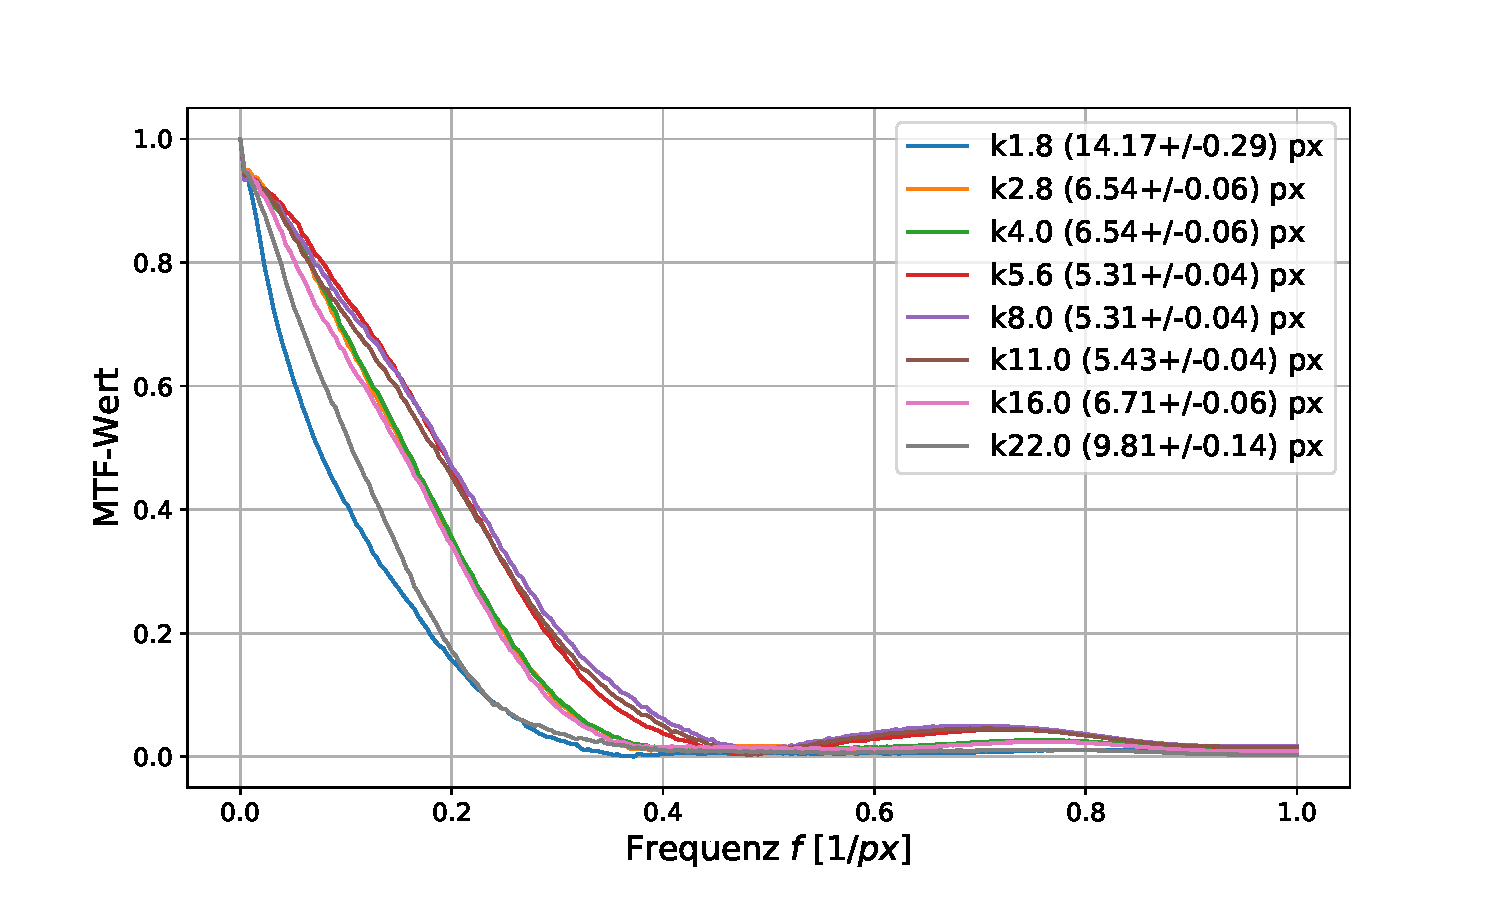
\includegraphics[width=1\textwidth]{data/kStufen.pdf}
			\caption{MTF-Kurven aller 8 Blendenzahlen $k$ sowie die Halbwertsfrequenzen dieser. Ein rascher Abfall bedeutet, dass dem Bild die hohen Frequenzen fehlen und so scharfe Kanten nicht abgebildet werden können. Eine hohe Halbwertsfrequenz zieht also eine hohe Schärfe und Qualität mit sich. Das schärfste Bild wurde somit mit $k=5,6$ bis $k = 8$ geschossen.}
			\label{fig:kStufen}	
		\end{figure}
		Bei der Grenzfrequenz $f_{1/2}$ ist der MTF-Wert auf die Hälfte abgefallen.
		Diese Frequenzen sind in Abhängigkeit der Blendenzahl $k$ in Abb. \ref{fig:kStufen} dargestellt.
		Aus dieser Abbildung lässt sich entnehmen, dass die Grenzfrequenz zwischen $k = 5,6$ und $k = 8,0$ am höchsten sein muss.
		\begin{figure}[ht]
			\centering
			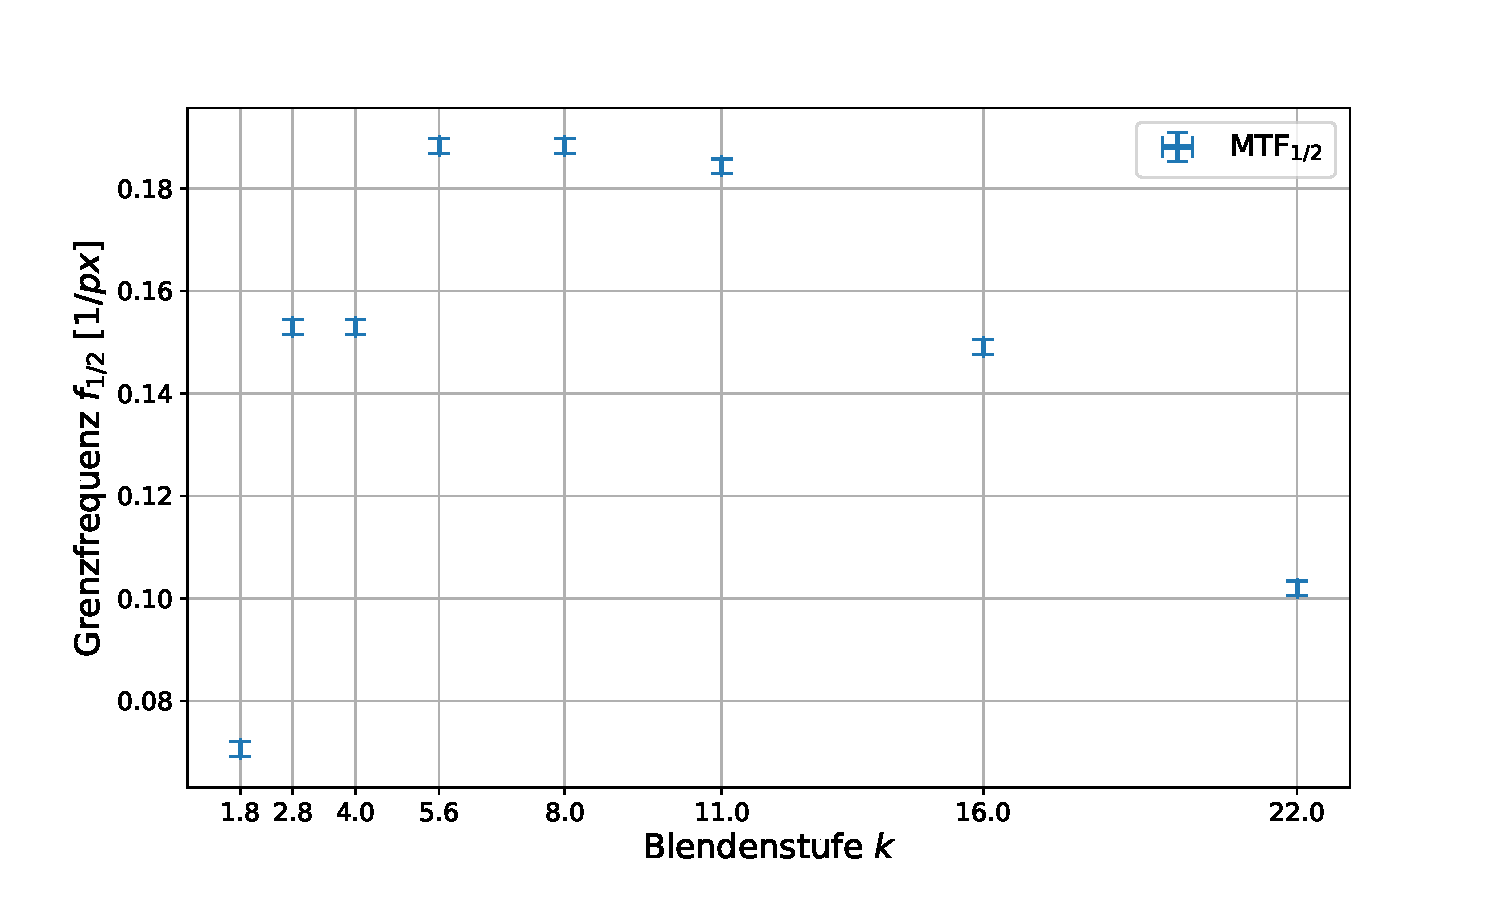
\includegraphics[width=1\textwidth]{data/kHalbe.pdf}
			\caption{Die Halbwertsfrequenz aufgetragen gegen die Blendenzahl $k$. Der Hochpunkt bei $k = 8$ ist der Punkt des schärfsten Bildes.}
			\label{fig:kHalbe}	
		\end{figure}
	
	\subsection{Auflösung bei der Einzellinse}

		\subsubsection{einfache Blenden}
						
			\begin{figure}[ht]
				\centering
				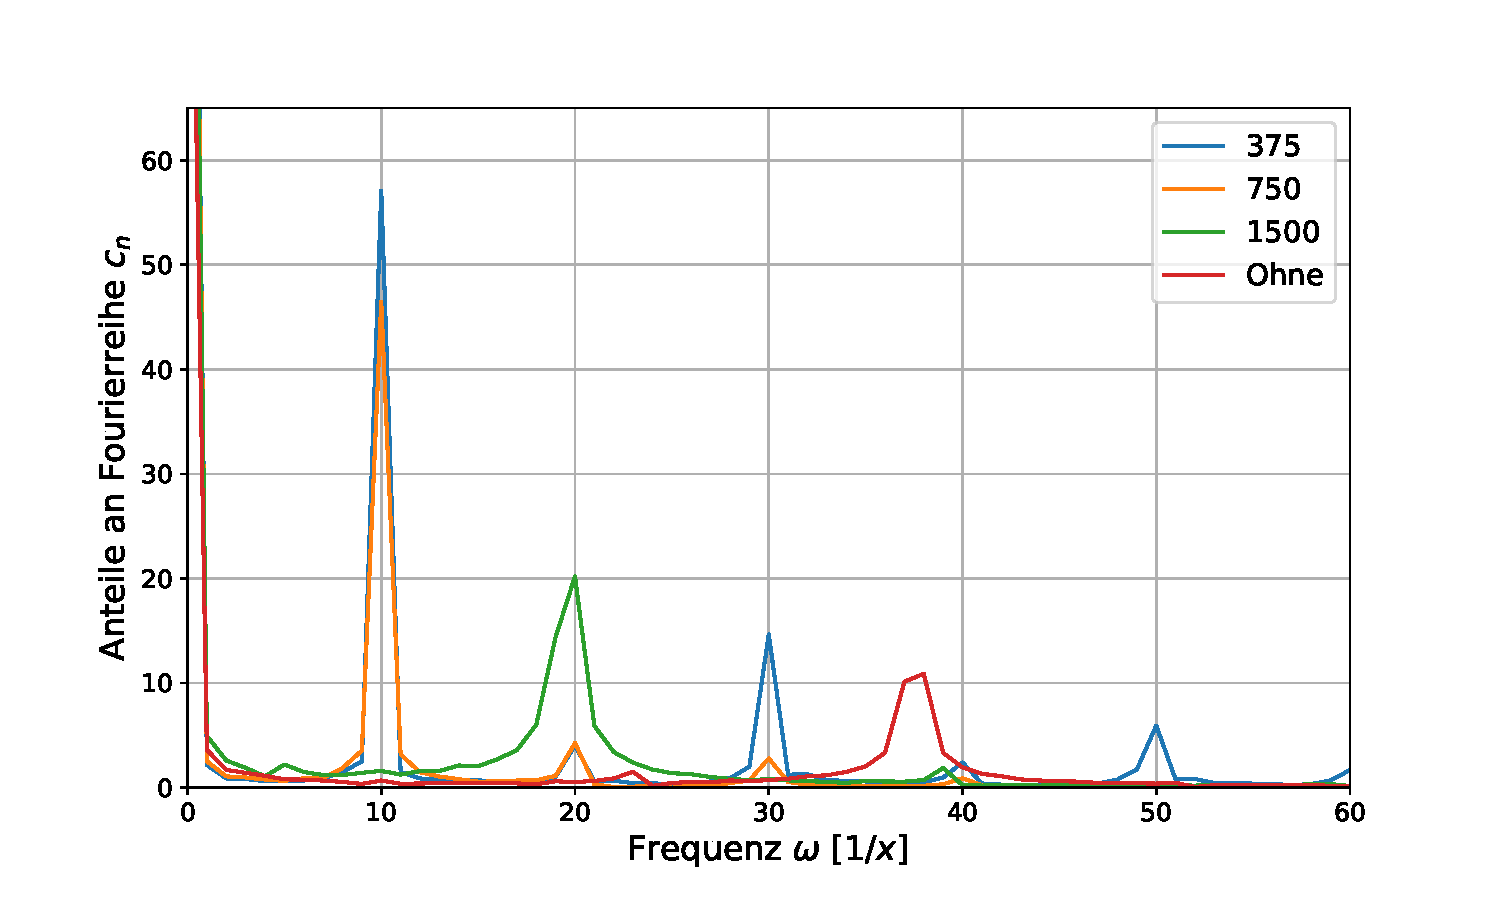
\includegraphics[width=1\textwidth]{data/FFTLinie1.pdf}
				\caption{Die Frequenzen der breiten Streifenpaare aller vier Blenden. Diese wurden mittels FFT bestimmt. Die Peaks aller Blenden sind erkennbar.}
				\label{fig:FFT1}
			\end{figure}
			
			\begin{figure}[ht]
				\centering
				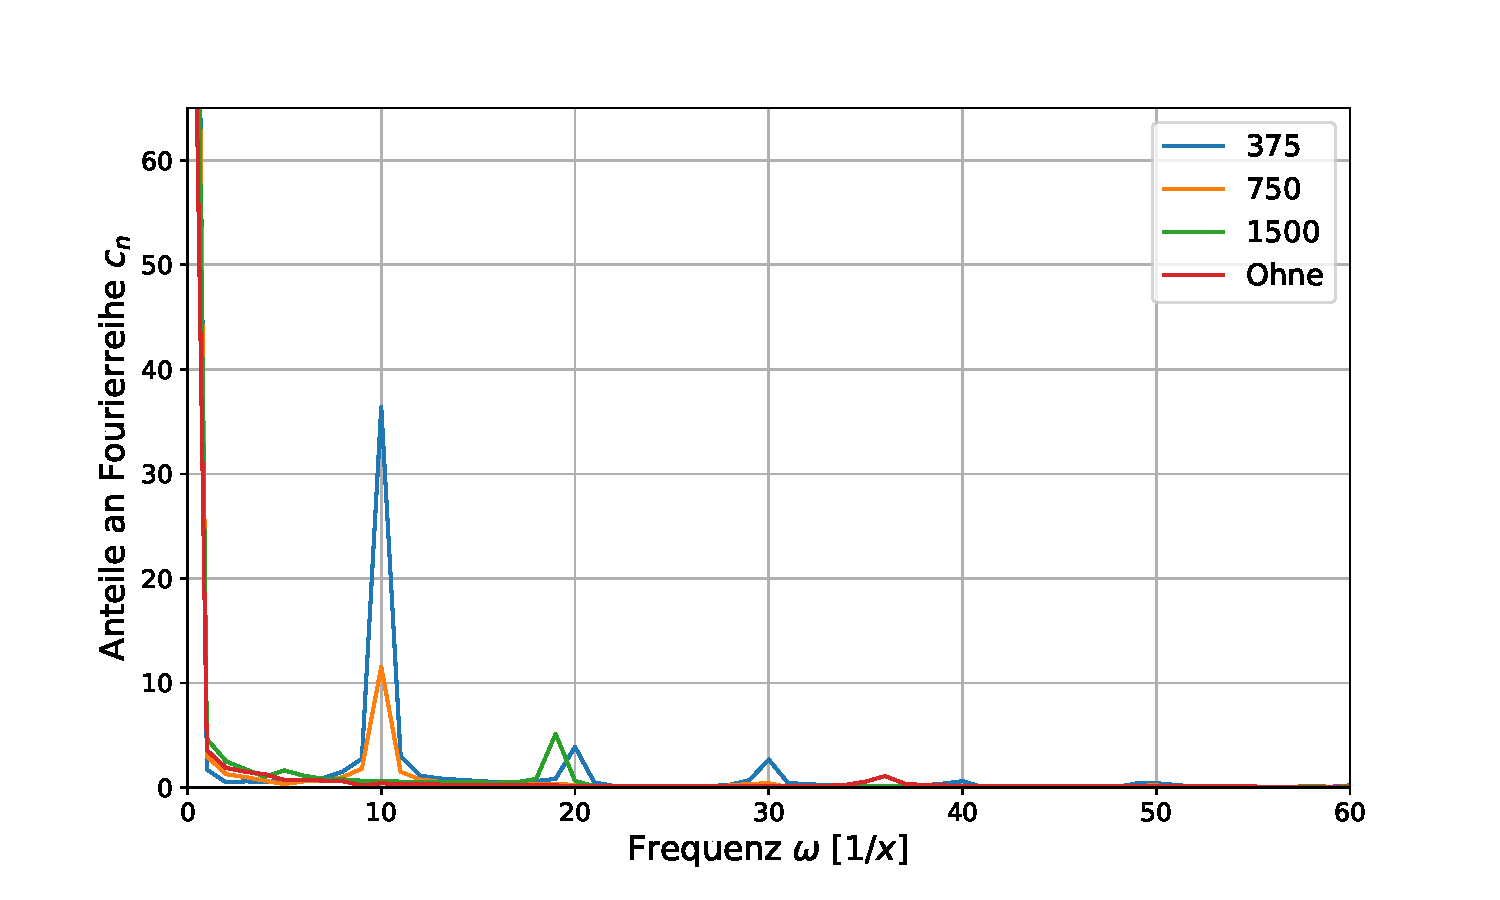
\includegraphics[width=1\textwidth]{data/FFTLinie4.pdf}
				\caption{Die Frequenzen der engsten Streifenpaare aller vier Blenden. Im Vergleich zu Abb. \ref{fig:FFT1} sind diese deutlich kleiner und reichen nicht mehr so weit in den Frequenzraum hinein.}
				\label{fig:FFT2}	
			\end{figure}
			
			\begin{figure}[ht]
				\centering
				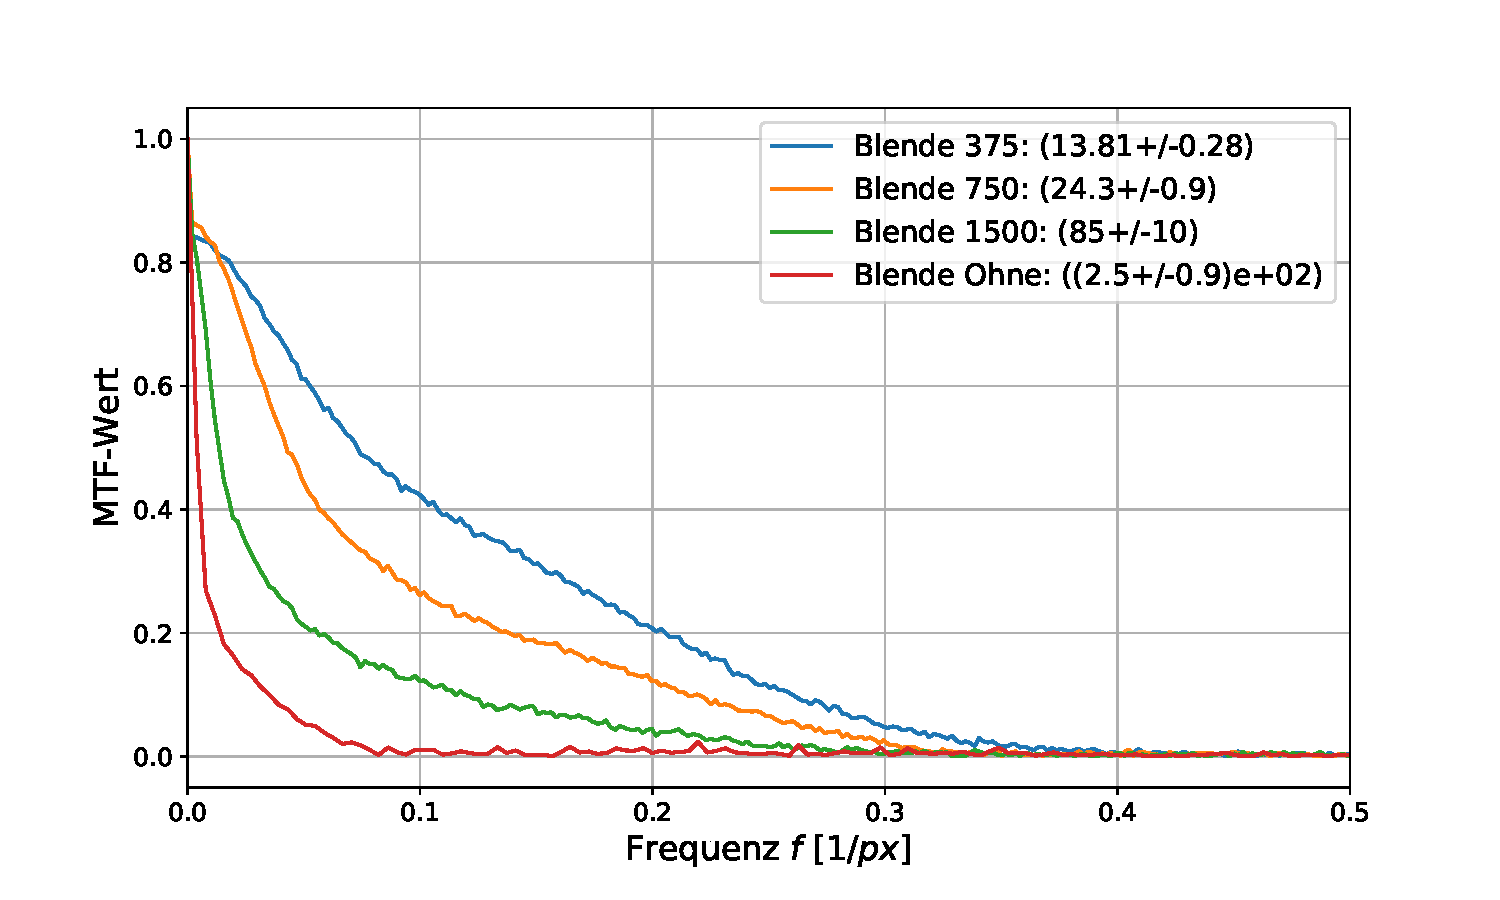
\includegraphics[width=1\textwidth]{data/MTFKanteLinsen.pdf}
				\caption{Die MTF-Kurven für die Einzelblenden. Dabei ist die Halbwertsbreite in Pixeln angegeben, was das Auflösungsvermögen bestimmt. Je höher diese Halbwertsbreite ist, desto größer die Auflösung.}
				\label{fig:MTF}	
			\end{figure}
					
			\begin{figure}[ht]
				\centering
				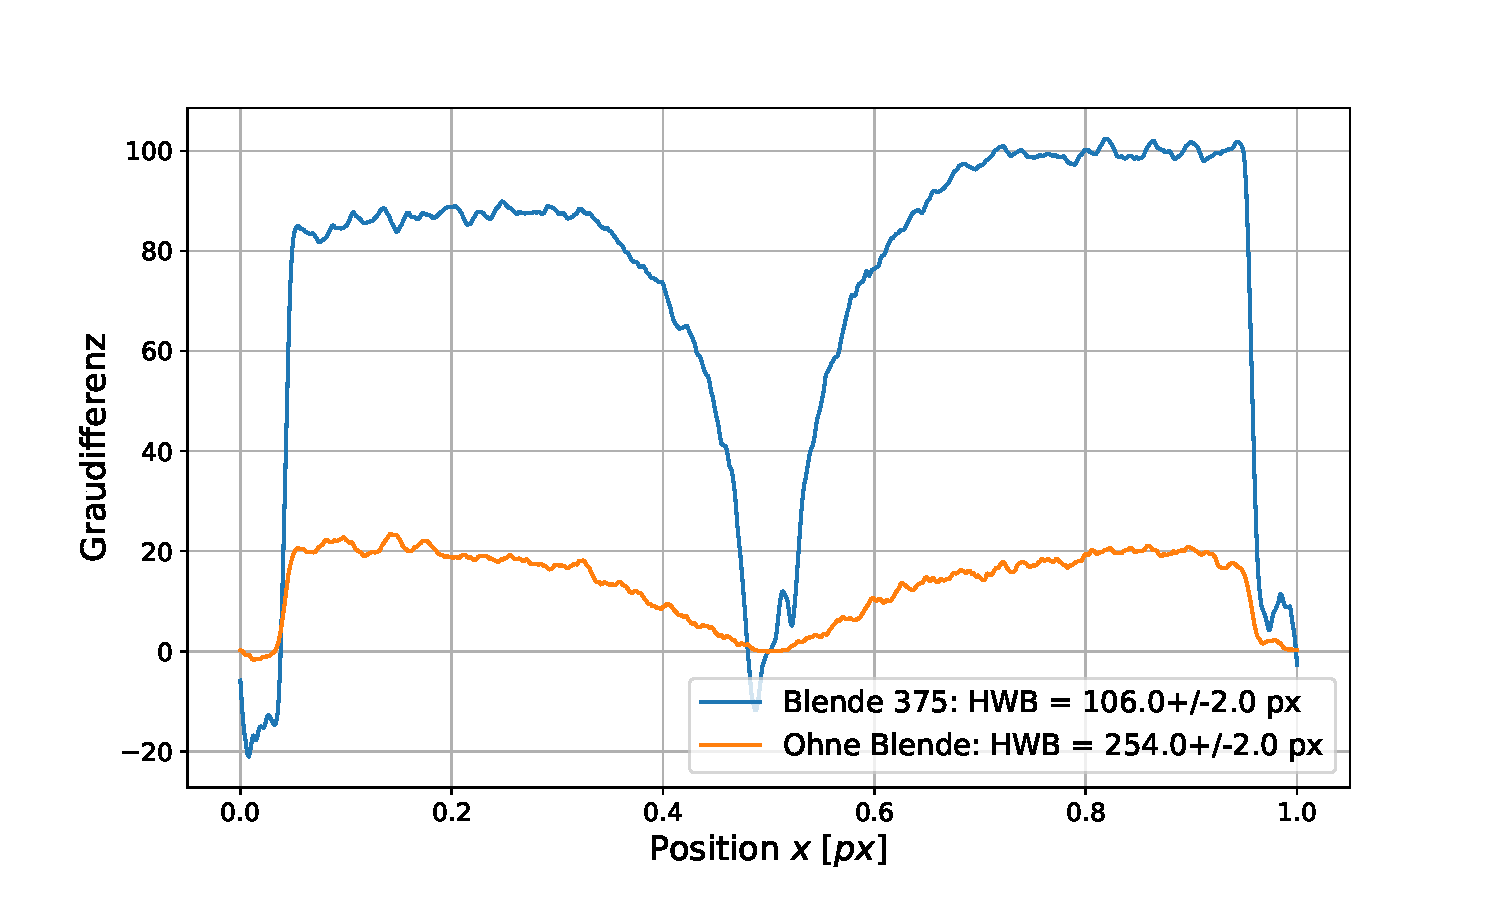
\includegraphics[width=1\textwidth]{data/Sterne.pdf}
				\caption{Differenz der Grauwerte von einem Profil durch ein weißes und ein Profil durch ein schwarzes Segment.
					 Dargestellt sind die beiden Profile der \SI{3.75}{\milli\meter}-Blende und des Fotos ohne Blende.
					 Am Rand des Siemenssternes treten Störungen auf.
					 In der Mitte liegt ein nicht eingefärbtes weißes Gebiet, weshalb die Differenz hier null wird.
					 Die Werte wurden in ihrer Umgebung gemittelt, um Rauschen zu unterdrücken.
					 Die kleinere Blende hat allgemein eine deutlich höhere Differenz, also einen höheren Kontrast.
					 Zusätzlich fällt die Differenz in Richtung Mitte nicht so schnell ab und die Halbwertsbreite ist so kleiner, was auf einen schärferen Ubergang und somit höhere Auflösung hindeutet.
				\label{fig:Sterne1}	
			\end{figure}
		
			%TODO kann sein das das wo anders hin kommt
			Die in Abb. \ref{fig:FFT2} gezeigten Frequenzen deuten darauf hin, dass die Streifen nicht mehr gut aufgelöst werden können.
			Die Peaks für $d = \SI{3.75}{\milli\meter}$ und $d = \SI{7.5}{\milli\meter}$ sind deutlich kleiner als in Abb. \ref{fig:FFT1} und für größere $d$ lassen diese sich fast nicht mehr ausmachen.
			Das die Frequenzen nicht mehr so weit in den Frequenzraum ragen, deutet auf einen weicheren Übergang zwischen den einzelnen Streifen hin, also einem Verwischen der Bereiche.
			Die kleinste Blende weist hier den größten Peak und den kleinsten Abfall auf, also ist die Auflösung mit dieser Blende am höchsten.
			
			In Abb. \ref{fig:MTF} sind die MTF-Kurven für die vier verschiedenen Blenden angegeben.
			Man kann wie erwartet sehen, dass die \SI{3.75}{\milli\meter}-Blende das beste Auflösungsvermögen zeigt.
			Dies untermauert obige Aussage, dass diese Blende die höchste Auflösung ermöglicht.
			
		\subsubsection{Lochblende}
			
			\begin{figure}[ht]
				\centering
				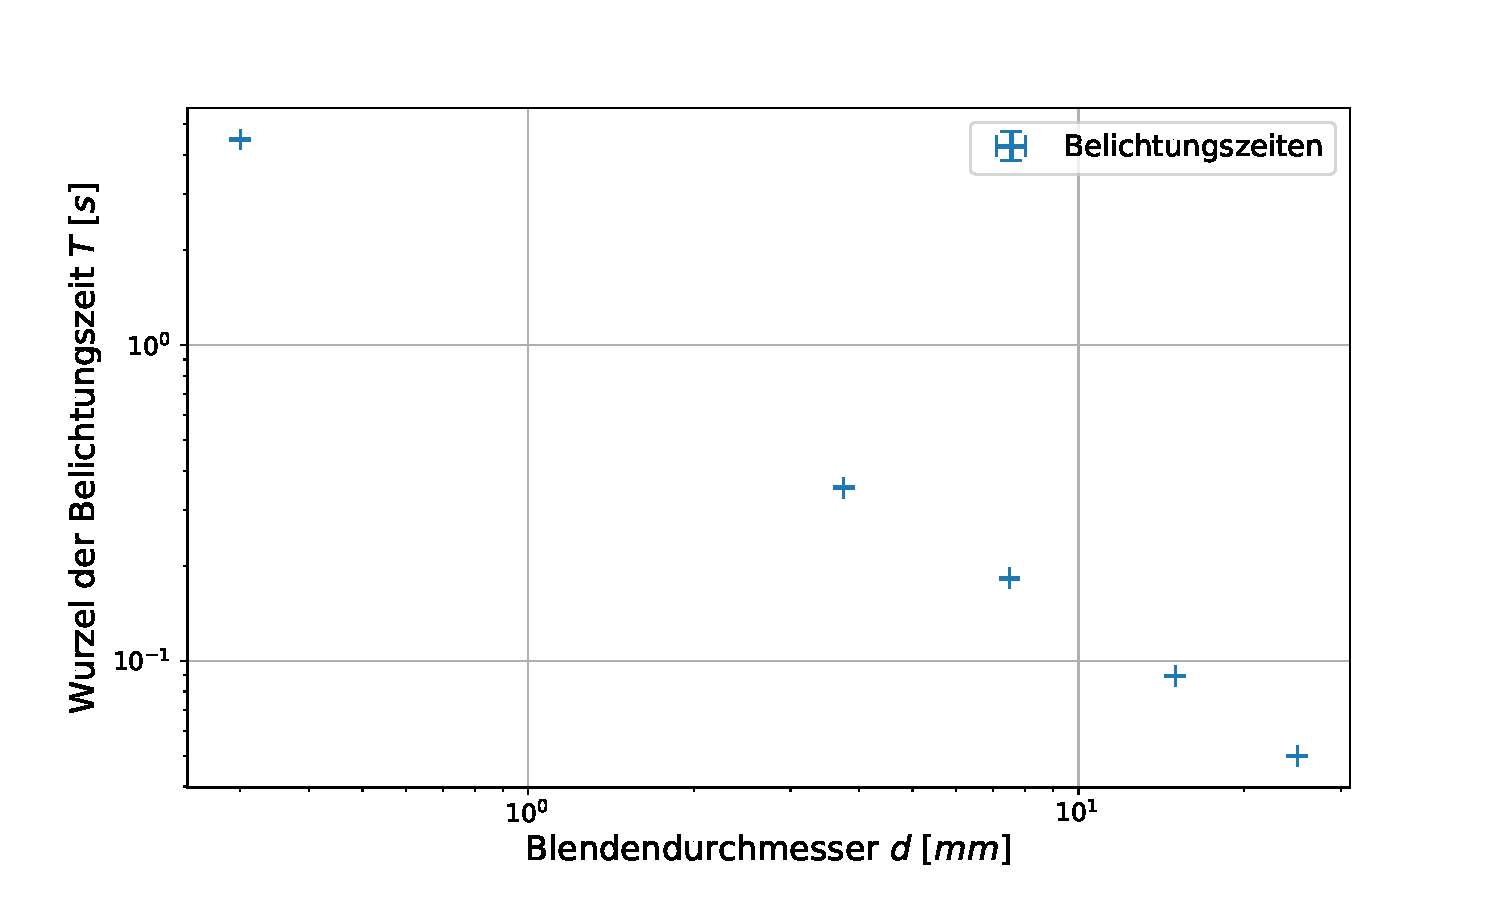
\includegraphics[width=1\textwidth]{data/Zeitvergleich.pdf}
				\caption{Die Belichtungszeit gegen den Blendendurchmesser aufgetragen. Die Achsen sind logarithmisch skalliert. Es folgt ein linearer Verlauf und der Blendendurchmesser der Lochblende kann etwa auf \SI{0.3}{\milli\meter} abgeschätzt werden.
				\label{fig:Belichtung}	
			\end{figure}
			
			% TODO
	
	% Datenanalyse:
	% - alle Messungen darstellen
	% - wichtige Beobachtungen beschreiben (Bedeutung dieser erklären)
	% - Aufführung der Formeln/Rechnungen zur Datenanalyse (nachvollziehbar ~ Quellen)
	% - Alle Originaldaten zur Verfügung stellen (~ Laborbuch)
		
\section{Diskussion}
	
	% TODO
	% Bezug:
	% - Rückgriff auf Hypothese/Problemstellung (Unterstützung?)
	% - Rolle der Ergebnisse in der Bewertung einbringen
	% 
	% Argumentation:
	% - Daten/Ergebnisse überzeugend für Argumentation verwenden
	% 
	% Logik: 
	% - Schlussfolgerungen logisch aus den Daten/Ergebnisse und Vorwissen ziehen
	% 
	% Unsicherheiten:
	% - Quellen für Unsicherheiten identifizieren
	% - Auswirkungen dieser auf Ergebnisse erläutern
	% 
	% Zusammenhang:
	% - Ergebnisse in wissenschaftlichen Kontext einordnen
	% - Auswirkungen diskutieren
	% - weiterführende Unterstützungen oder Verbesserungen vorschlagen